\documentclass[upLaTex, 10pt,dvipdfmx,a4paper,twocolumn]{jsarticle}
% \documentclass[upLaTex,dvipdfmx,a4paper,twocolumn,base=15pt,jbase=15pt,ja=standard]{jsarticle}
\usepackage[margin=20mm]{geometry}
\usepackage[dvipdfmx]{graphicx}
\usepackage[dvipdfmx]{color}
\usepackage{float}
% \usepackage{ipsj}
% \usepackage{amsmath}
% \usepackage{mathtools}
% \usepackage{showon??__}

\begin{document}

% ここのタイトルは後ほど修正
% 話題遷移について書いてみる ver
\title{発話の機能を考慮した雑談対話システムにおける不適切な話題遷移の検出}
\author{初田 玲音}
\date{2021年 11月 8日 中間発表}


\maketitle

\section{研究背景}
    近年,雑談対話システムの研究が盛んである.雑談では,ユーザは明確な目的もなく,自由に発話を行うため,対話システムが自然に対話を続ける為には,多様な話題に対応することに加え,その話題を自然な範囲内で展開及び遷移することが求められる.\\
     しかし,現在の対話システムでは,適切な応答を出力し続けることは困難であり,対話破綻を引き起こす発話をすることがある.この対話破綻を引き起こす発話のうち,不適切な話題遷移が原因である発話を,本研究では不適切な話題遷移とする.不適切な話題遷移によって,ユーザの対話意欲を喪失し,対話の継続が困難になることが考えられるため,このような発話を事前に検出し,抑制することは重要である.従来においても,不適切な話題遷移を検出する研究は存在するが,word2vec\cite{w2v} で得られる分散表現のみを考慮しており,対話における発話の機能を考慮していない.\\
     そこで本研究では,話題遷移の特性と,発話の機能を考慮した特徴量を提案し,従来の方法と比較してその有効性を検証することを目的とする.
     
\section{関連研究}
    話題遷移を考慮した対話破綻検出として,Sugiyama\cite{sugiyama}の研究がある.Sugiyama は,話題遷移の自然さを捉える特徴として,システム発話と直前のユーザ発話との単語類似度や,対話行為や発話文の長さなどを導入した.それらの特徴量を基に,回帰分析手法のスタッキングを用いてアンサンブルすることで,DBDC3において,最も高い精度を得た.この手法では,対話行為等の様々な特徴が導入されたが,学習データ及び評価データは,原因が不適切な話題遷移ではない対話破綻を含んでいる為,どのような話題遷移の検出に対して有効かは示されていない.\\
     破綻した話題遷移の検出として,豊嶋ら\cite{toyoshima}の研究がある.豊嶋らは,システムの破綻した話題遷移を検出することを目的として,システム発話と,その直前のユーザ発話を, word2vec を用いて発話ベクトルを算出し,発話ベクトルの差分情報を基に対話破綻を検出する手法を提案した.この手法では,明らかに破綻した話題遷移の検出率は高いが,発話ベクトルのみを考慮しているため,対話行為のような発話の役割については考慮されていない.\\

\section{提案手法}
    本節では,ユーザとシステムの2者対話列を入力とし,各対話において,ユーザ発話に対するシステム発話が不適切な話題遷移が否かを推定する提案手法について述べる.\\
     不適切な話題遷移は,直前のユーザ発話の話題に対して,表層的にも意味的にも関連しない話題を持つ発話である.しかし, Higashinakaらによれば,次のいずれかの場合は不適切な話題遷移としない.
    \begin{itemize}
        \item 直前のユーザ発話が後ろ向き機能を有し,システムが新たな話題を提供している
        \item システム発話が,直前のユーザ発話に対する後ろ向き機能を持つ発話と,新たな話題の提供を同時に行っている
        \item 直前のユーザ発話が,明確な話題を持たない
    \end{itemize}

    なお,後ろ向き機能とは,特定の応答を相手に対して働きかける前向き機能を有する発話に対して,応答,同意,理解,基盤化の機能を指す.\\
     提案モデルの全体像を図\ref{fig:all}に示す.

    \begin{figure}[htb]
        % \centering
        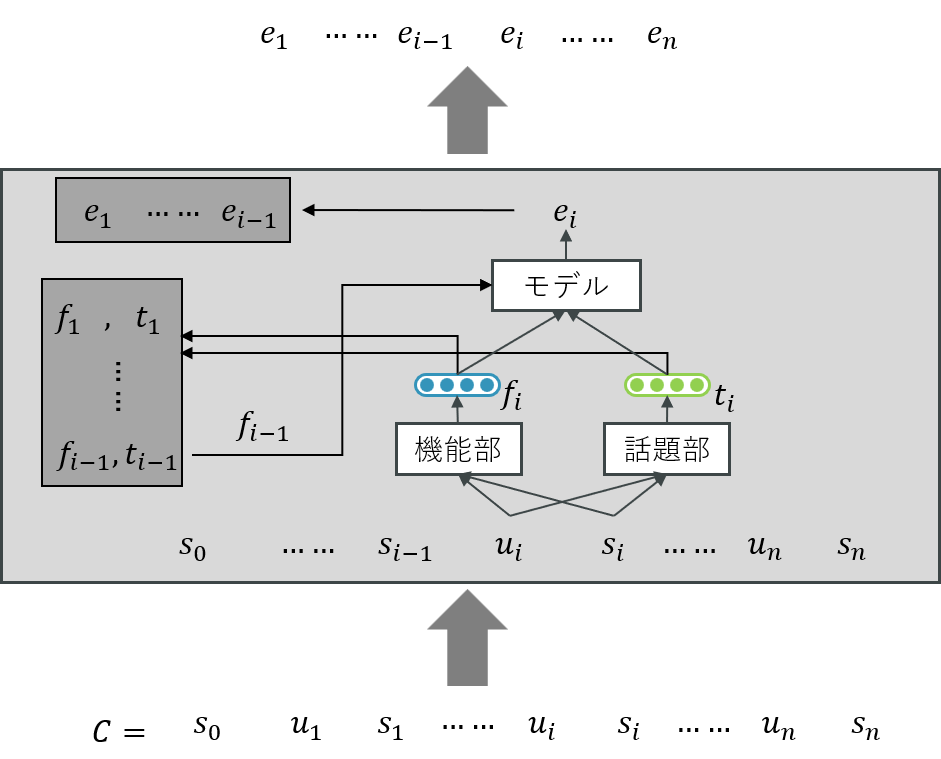
\includegraphics[keepaspectratio, scale=0.6]{ img/all.png }
        \caption{提案モデル 概略図}
        \label{fig:all}
    \end{figure}

    ユーザとシステムの2者対話全体を,
    \begin{equation}
    \label{convs}
        C = s_0, u_1, s_1, ..., u_i, s_i, ..., u_t, s_t
    \end{equation}
    と表す.(\ref{convs})式の $s_i$ はシステム発話, $u_i$ はユーザ発話を表し,$u_i, s_i$ のユーザ発話とシステム発話の1組を1つの対話とする.(\ref{convs})式では,開始のシステム発話 $s_0$ から始まり,$t$ 個の対話が続くことを示している.\\
     図\ref{fig:all}に示した提案システムでは,2者対話列を入力し,$u_i$と$s_i$を話題部,機能部によってそれぞれの特徴量$t_i, f_i$を抽出する.次に,得られた特徴量と,$f_(i-1)$を識別モデルに入力し,2値分類の出力 $e_i$ を得る.以上の処理を$n$回行い,最後に推定結果として$e_1, ..., e_i, ..., e_n$ を出力する.

    \subsection{話題部}
    本節では,提案手法における話題部で検討している各特徴量について述べる.以下の特徴量を全て連結して,話題ベクトル$t_i$を得る.話題部では,ユーザの発話とシステム発話の発話ベクトルから,発話内容の関連性を表現する特徴量を抽出する.
    \subsubsection{差分ベクトル}
        豊島\cite{toyoshima}らと同様に,各発話に対して形態素解析を行い,その品詞情報に基づいて内容語(名詞,動詞,形容詞)を抽出した.なお,本実験では,形態素解析に ginza を用いる.次に,抽出した内容語に対応する分散表現の総和を,ノルムで正規化した値を算出し,それを発話ベクトルとする.最後に,ユーザ発話とシステム発話のそれぞれの発話ベクトルの差を取り,それを差分ベクトルとする.本実験では,ginza の分散表現を用いる.差分ベクトルを特徴量とすることで,明らかに破綻した話題遷移の検出を期待する.
    \subsubsection{差分ベクトルのノルム}
        差分ベクトルのノルムが小さい場合は,ユーザの発話ベクトルとシステム発話ベクトルの差が小さい為,話題が大きく遷移していない事が期待出来る.差分ベクトルのノルムが大きい場合は,強い話題遷移か,ユーザ発話かシステム発話のどちらかが,明確な話題を持たないことを表現すると考えられる.
    \subsubsection{自己相互情報量}
        ユーザ発話に含まれる語と,システム発話に含まれる語が表層的に全く異なっていても,意味上では常識の範囲で遷移している場合が考えられる.自己相互情報量を導入することで,共起のしやすさを,即ち話題遷移の自然性を考慮すると期待する.
     
    \subsection{機能部}
    本節では,提案手法における機能部で検討している各特徴量について述べる.以下の特徴量を全て連結して,機能ベクトル$f_i$を得る.機能部では,発話の表層から,前向き機能と後ろ向き機能の分類に有効な特徴量を抽出する.
    \subsubsection{N-graam}
        発話内容を表し,機能の分類に有効と考えられる素性である.文末表現や,付属語列も分類に有効と考えられる為,内容語を全て品詞で正規化した N-gram も導入する.本研究では,N=1,2,3 を検討している.
    \subsubsection{キーワード}
        特定機能の分類に有効なキーワードを選定する.このキーワードの決定方法については,検討中である.

    % \subsection{データ}
    % 学習データ及び評価データとして, Higashinaka らが作成した,対話破綻エラー類型分類がアノテーションされたデータセットを用いる\cite{araki}.このデータセットは,過去の対話破綻検出チャレンジ(Dialogue Breakdown Detection Challenge: DBDC)\cite{higashinaka}で収集されたデータセットに対して,対話破綻とされたシステム発話に,17種の対話破綻の原因がアノテーションされたものであり,[文脈-形式]軸で定義された話題遷移エラーを用いる.

\section{評価方法}
    Sugiyamaらの手法をベースラインとして,提案手法の結果の比較を検討している.また,全ての特徴量を用いた結果から,ある特徴量を用いなかった場合の結果を差し引くことで,提案したどの特徴量が効果的であったかを検証することを検討している.

\section{今後の課題}
 \begin{itemize}
     \item 前向き機能,後ろ向き機能のアノテーション
     \item 具体的な学習モデルの決定
     \item 実験方法,評価方法について検討する
 \end{itemize} 

 
 
\begin{thebibliography}{99}
    \bibitem{w2v} Tomas Mikolov, Ilya Sutskever, Kai Chen, Greg Corrado, and Jeffrey Dean. Distributed representations of words and phrases and their compositionality. In NIPS, 2013.
    \bibitem{higashinaka} 東中竜一郎,船越孝太郎,小林優佳,稲葉通将 : 対話破綻検出チャレンジ. 第75回言語・音声理解と対話処理研究会(第6回対話システムシンポジウム),人工知能学会研究会資料 SIG-SLUD-75-B502,pp. 27-32(2015)
    \bibitem{araki} Ryuichiro Higashinaka, Masahiro Araki, Hiroshi Tsukahara and Masahiro Mizukami:Integrated taxonomy of errors in chat-oriented dialogue systems,  SIGDIAL 2021.
    \bibitem{sugiyama} Hiroaki Sugiyama. Dialogue breakdown detection based on estimating appropriateness of topic transition. In Diaog System Technology Challenges 6, 2017.
    \bibitem{toyoshima} 豊嶋 章宏, 吉野 幸一郎, 須藤 克仁, 中村 哲 : 発話ベクトルの差分特徴量を用いた雑談対話システムにおける破綻した話題遷移の検出, 言語処理学会 第24回年次大会, p873-p873
    % \bibitem{hori} 堀井朋,森秀晃,林卓也,荒木雅弘: 破綻類型情報に基づく雑談対話破綻検出, 言語・音声理解と対話処理研究会,vol.78, pp.75-80, 2016
    % \bibitem{K}Khatri C, Hedayatnia B, Goel R, Venkatesh A, Gabriel R, Mandal A. Detecting Offensive Content in Open-domain Conversations using Two Stage Semi-supervision. In: Proceedings of the 32nd Conference on Neural Information Processing Systems (NeurIPS); 2018. p. 1–9. 


\end{thebibliography}

\end{document}